\documentclass{article}

\usepackage[margin=1in]{geometry}
\usepackage{booktabs}
\usepackage{listings}
\usepackage{xcolor}
\usepackage[hidelinks]{hyperref}
% \usepackage{microtype} % disabled: font expansion error in this environment
\usepackage{amsmath}
\usepackage{amssymb}
\usepackage{float}
\usepackage{fancyhdr}
\usepackage{mdframed}
\usepackage{parskip}
\usepackage{setspace}
\usepackage{tikz}
\usetikzlibrary{shapes.geometric, arrows.meta, positioning}

\lstset{
  basicstyle=\ttfamily\small,
  breaklines=true,
  frame=single,
  backgroundcolor=\color{gray!10}
}

\pagestyle{fancy}
\fancyhf{}
\fancyhead[L]{\small LICITRA-TR-2026-01 \quad v0.2}
\fancyhead[R]{\small Nutalapati (2026)}
\fancyfoot[C]{\thepage}
\renewcommand{\headrulewidth}{0.4pt}

\title{%
  \textbf{LICITRA-MMR: A Merkle Mountain Range Ledger Primitive for}\\[0.3em]
  \textbf{Cryptographic Runtime Accountability in Agentic AI Systems}\\[16pt]
  \normalsize\textsc{LICITRA Technical Report Series}\\[4pt]
  \normalsize Report No.\ \textbf{LICITRA-TR-2026-01}
  \quad Version \textbf{0.2} \quad March 2026
}

\author{%
  Narendra Kumar Nutalapati\\[0.3em]
  \small Independent Researcher\\
  \small Portland, Oregon, USA\\
  \small \href{mailto:narendrakumar.nutalapati@gmail.com}%
    {narendrakumar.nutalapati@gmail.com}
}

\date{March 2026}

\begin{document}
\maketitle
\thispagestyle{fancy}

\begin{center}
\begin{tabular}{@{}ll@{}}
\toprule
\textbf{Report number}    & LICITRA-TR-2026-01 \\
\textbf{Version}           & 0.2 \\
\textbf{Date}              & March 2026 \\
\textbf{Commit}            & \texttt{70ec6e4} \\
\textbf{Repository}        & \url{https://github.com/narendrakumarnutalapati/licitra-mmr-core} \\
\textbf{Code archive DOI}  & \url{https://doi.org/10.5281/zenodo.18796529} \\
\textbf{Report DOI}        & \url{https://doi.org/10.5281/zenodo.18843032} \\
\textbf{License (code)}    & MIT \\
\textbf{License (report)}  & CC BY 4.0 \\
\bottomrule
\end{tabular}
\end{center}

\bigskip

\begin{abstract}
\noindent
Agentic AI systems that make autonomous decisions in production create a
new class of accountability requirement: the ability to reconstruct, after
the fact, the exact decision chain with cryptographic verifiability---a
stronger guarantee than operational logs alone provide. Existing logging
approaches---including mutable database logs, hash chains, and
general-purpose tamper-evident stores not tailored for agentic
governance---provide observability but do not address independently
verifiable runtime decision chains. This report documents LICITRA-MMR, an
open-source ledger primitive that combines a Merkle Mountain Range (MMR)
data structure with per-organization epoch anchoring, a versioned canonical
JSON specification, and an atomic two-phase commit pipeline. At a block
size of 1,000 events, LICITRA-MMR produces inclusion proofs requiring 14
SHA-256 operations, verifies a full epoch chain of 1,000 epochs in under
1~ms, and supports full leaf rehash of 1 million events in approximately
2~seconds. The system is fully open-source under MIT license with a tagged
release, reproducible test suite (11/11 passing), and evidence bundles.
LICITRA-MMR is a single-operator forensic integrity primitive: it provides
no Byzantine fault tolerance, no distributed consensus, and no
confidentiality guarantees. All performance figures in this report are
analytical estimates derived from SHA-256 microbenchmark component
latencies; no production benchmarking under concurrent workload has yet
been performed. This document is a versioned archival technical report of
the reference implementation at release v0.1.0-mvp.
\end{abstract}

\medskip
\noindent\textbf{Keywords:} Merkle Mountain Range, agentic AI, cryptographic
audit, runtime integrity, tamper-evident logging, AI governance

\bigskip\hrule\bigskip
\tableofcontents
\bigskip\hrule\bigskip

%%─────────────────────────────────────────────────────────────────────────────
\section{Introduction}

Regulatory frameworks for high-risk AI systems are increasing operational
pressure toward stronger audit guarantees for autonomous decision chains.
The EU AI Act Article~12~\cite{euaiact} requires that high-risk AI systems
generate logs that are traceable and sufficient for post-market monitoring.
The Colorado AI Act~\cite{coloradoai} (SB~24-205, effective June~30, 2026)
requires deployers to document AI decision-making processes and conduct impact
assessments. These frameworks increase demand for verifiable logging mechanisms
that most production agentic AI stacks do not currently provide. LICITRA-MMR
does not claim to satisfy any specific regulatory mandate; it provides a
technical primitive consistent with the audit integrity goals such frameworks
express.

The gap is primarily technical rather than conceptual. Most teams deploy
agentic AI with mutable database logs, cloud logging pipelines, or
dashboard-based observability. These systems answer the question: \textit{what
does our log say happened?} They do not answer: \textit{can we prove the log
was not modified after the incident?} The distinction matters because
administrators can rewrite database rows, cloud logs can be truncated or
filtered, and cleanup scripts can alter historical records. A post-incident
forensic investigation that relies entirely on operator-controlled logs provides
no independent verification guarantee.

Agentic systems intensify this problem. Unlike single-inference ML systems,
autonomous agents make multi-step decisions---each step potentially triggering
real-world actions---without per-action human oversight. The decision chain
that produced a harmful outcome may span dozens of sequential operations, each
dependent on prior context. Reconstructing that chain requires not just that
each event was logged, but that the sequence is complete, ordered, and
unmodified.

This report documents the following contributions of the LICITRA-MMR reference
implementation:

\begin{enumerate}
\item \textbf{Canonical JSON Specification.} A versioned, cross-implementation
  deterministic serialization format (CANONICAL\_JSON\_SPEC v1.0) that ensures
  identical byte sequences from identical logical payloads across independent
  implementations---a prerequisite for deterministic verification.

\item \textbf{MMR-Based Per-Organization Tamper-Evident Ledger.} A Merkle
  Mountain Range data structure providing $O(\log n)$ inclusion proofs and
  append-only semantics, with per-organization epoch anchoring that chains
  epoch roots into a hash-linked sequence resistant to retroactive modification.

\item \textbf{Atomic Two-Phase Commit Pipeline.} A propose~$\to$~policy~$\to$
  commit pipeline in which every MMR append, event record, and epoch
  finalization occurs within a single database transaction, preventing partial
  writes that could leave the ledger in an inconsistent state.

\item \textbf{Open-Source Implementation with Reproducible Evidence.} A fully
  tested (11/11 passing), MIT-licensed implementation at tagged release
  v0.1.0-mvp, with reproducible JSON evidence bundles covering five
  tamper-detection scenarios.
\end{enumerate}

\noindent This work should be understood as an applied cryptographic systems
design contribution---specifically, an authenticated data structure engineering
effort targeting agentic AI governance infrastructure---rather than a novel
cryptographic primitive or consensus protocol.

%%─────────────────────────────────────────────────────────────────────────────
\section{Background}

\subsection{Merkle Mountain Ranges}

A Merkle Mountain Range is an append-only authenticated data structure
introduced by Peter Todd in the context of Bitcoin timestamping~\cite{todd2013}.
Unlike many Merkle tree implementations, in which insertion requires updating
internal nodes along the rightmost path, an MMR avoids modifying previously
committed subtrees. It maintains a forest of perfect binary trees (peaks) that
are merged as new leaves are appended. This property makes MMRs suitable for
append-only audit logs: each new element extends the structure in $O(\log n)$
time and space without modifying any existing node.

Formally, an MMR of size $n$ stores $2n - \text{popcount}(n)$ nodes, where
$\text{popcount}(n)$ is the number of set bits in the binary representation of
$n$. The peaks of the MMR are the roots of the constituent perfect binary trees.
A single MMR root is produced by \emph{bagging} the peaks: hashing them
right-to-left into a single digest. An inclusion proof for a leaf at position
$p$ consists of the sibling hashes on the path from $p$ to its subtree peak,
plus the remaining peaks, enabling logarithmic verification without access to
the full node set.

At \textsc{block\_size}~$= 1{,}000$ (the default epoch size), the MMR contains
1,994 nodes and produces inclusion proofs requiring exactly 14 hash operations.
A standard balanced Merkle tree over the same leaf count requires
$\lceil\log_2(1000)\rceil = 10$ hashes per proof path but requires updating
internal nodes on insertion. The formal optimality of the MMR for append-only
accumulators was established by Bonneau et al.~\cite{bonneau2025}.

\subsection{Epoch Anchoring}

LICITRA-MMR partitions the event stream into fixed-size epochs of
\textsc{block\_size} events. When an epoch reaches capacity, an epoch record is
finalized containing:

\begin{lstlisting}
epoch_hash = SHA-256(
  prev_epoch_hash
  || mmr_root
  || SHA-256(metadata))
\end{lstlisting}

where \texttt{prev\_epoch\_hash} is the hash of the preceding epoch (or a
32-byte genesis value for epoch~0), \texttt{mmr\_root} is the bagged peak hash
of the epoch's MMR, and \texttt{metadata} is a canonical JSON document
containing the organization ID, epoch ID, sequence range, event count, and
ledger version.

This construction chains epochs into a hash-linked sequence analogous to a
blockchain header chain, without distributed consensus overhead. Modifying any
event within an epoch invalidates that epoch's MMR root, which invalidates all
subsequent epoch hashes. An auditor who holds the current epoch hash and any
historical event can verify the complete chain of custody from genesis to
present.

\subsection{The Agentic AI Accountability Gap}

Contemporary agentic AI systems---systems that autonomously plan and execute
multi-step tasks using large language models as reasoning engines---introduce
accountability challenges not present in traditional ML deployments. In a
single-inference deployment, a harmful output is a discrete event that can be
logged with a timestamp and input/output pair. In an agentic system, a harmful
outcome may result from a sequence of individually benign decisions that
collectively produce an unintended effect. Attributing the outcome requires
reconstructing the full decision chain: which prompts the agent saw, which tools
it invoked, which intermediate results it relied upon, and which final action it
executed.

Existing logging infrastructure is not designed for this requirement. Application
logs capture events as they occur but provide no tamper-evidence guarantees.
Observability platforms aggregate telemetry but rely on operator-controlled
infrastructure. Neither provides the forensic integrity consistent with emerging
AI regulation: the ability for an external party to verify, independently of
the operator, that a complete and unmodified record of the decision chain exists.

%%─────────────────────────────────────────────────────────────────────────────
\section{Threat Model}

LICITRA-MMR is designed to protect the integrity of an append-only audit ledger
against post-hoc modification. This section identifies the attacker classes
addressed and explicitly states what the system does and does not protect
against.

\subsection{Protected Against}

\textbf{T1 --- Insider / Database Administrator.} An attacker with direct write
access to the database attempts to modify the \texttt{canonical\_json} field of
a committed event. The leaf hash stored separately in the \texttt{leaf\_hash}
column will no longer match the recomputed SHA-256 of the modified canonical
JSON, and MMR verification will fail at the affected leaf position.

\textbf{T2 --- Log Scrubber / Row Deletion.} An attacker deletes one or more
event rows to suppress evidence of a specific decision. The monotonic
per-organization sequence number creates a detectable gap: verification will
identify missing sequence positions, and the MMR node set will contain orphaned
nodes at the deleted leaf positions.

\textbf{T3 --- Post-Incident Epoch Modification.} An attacker modifies a
historical epoch hash to hide evidence of prior tampering. Because each epoch
hash is computed over the previous epoch hash, any modification to a historical
epoch invalidates all subsequent epoch hashes.

\textbf{T4 --- Selective History Presentation.} An operator presents only a
subset of the audit log to an external auditor, claiming it is complete. An
independent auditor can verify completeness by recomputing the MMR root from the
presented events and checking it against the claimed epoch hash. Any omitted
events will produce a root mismatch.

\subsection{Not Protected Against}

\textbf{N1 --- Compromised Application Layer.} LICITRA-MMR commits whatever the
application layer submits. Pre-execution authorization integrity is outside the
scope of this system; see Section~\ref{sec:nongoals}.
LICITRA-SENTRY~\cite{licitrasentry} (LICITRA-TR-2026-02) addresses this gap with a
deterministic authorization control plane that commits every decision to LICITRA-MMR.

\textbf{N2 --- Unsigned Epoch Hashes.} The current implementation computes epoch
hashes but does not sign them with a private key. Ed25519 epoch signing is an
identified future extension; the epoch record schema reserves a
\texttt{signature} field for this purpose. See Section~\ref{sec:limitations}.

\textbf{N3 --- Availability Attacks.} LICITRA-MMR does not protect against
denial-of-service attacks against the underlying database or API layer.

\subsection{Trust Assumptions}

The system assumes: (1)~SHA-256 is collision-resistant; (2)~the database storage
layer preserves byte-level fidelity of stored values; (3)~at least one honest
party retains a copy of a recent epoch hash against which verification can be
anchored. Assumption~(3) is structurally equivalent to Certificate
Transparency's reliance on at least one honest log monitor~\cite{laurie2013}.
No assumption is made about the trustworthiness of the operator beyond
assumption~(2).

%%─────────────────────────────────────────────────────────────────────────────
\section{Trust Assumptions and Scope Limitations}
\label{sec:trustscope}

This section consolidates the system's scope boundaries for reference by
deployers and external auditors.

\textbf{Single-operator model.} LICITRA-MMR is designed for single-operator
deployments. There is one writer and one ledger per organization. Consistency
is enforced by database transaction semantics. Multi-party witnessing---where
independent operators each hold copies of current epoch hashes---is an
identified future architectural direction, analogous to the gossip protocol in
Certificate Transparency~\cite{laurie2013}.

\textbf{No Byzantine storage defense.} The system assumes the database storage
layer faithfully preserves byte-level fidelity of stored values. It does not
protect against a Byzantine storage layer that selectively corrupts data while
maintaining apparent internal consistency.

\textbf{No confidentiality guarantees.} LICITRA-MMR provides integrity and
tamper-evidence guarantees only. Encryption of event payloads is orthogonal to
the audit layer and is the responsibility of the application layer.

\textbf{Integrity guarantees depend on honest anchor holder.} The tamper-evidence
guarantees hold relative to at least one honest party retaining a copy of a
recent epoch hash. An adversary who controls both the database and all external
copies of prior epoch hashes could in principle reconstruct a consistent but
false history. This is the same foundational trust assumption as Certificate
Transparency~\cite{laurie2013}.

\textbf{No consensus protocol.} The epoch chain is structurally similar to a
blockchain header chain but is not a blockchain. There is no proof of work,
proof of stake, token, peer-to-peer network, or distributed ledger.

\textbf{No availability guarantee.} Availability is the responsibility of the
deployment infrastructure.

\textbf{No pre-execution authorization.} LICITRA-MMR records what was committed
to the ledger. It does not guarantee that what was committed accurately reflects
what the agent was authorized to do. Pre-execution authorization is outside the
scope of this system.

%%─────────────────────────────────────────────────────────────────────────────
\section{Security Properties}
\label{sec:security}

This section formalizes the core integrity guarantees provided by LICITRA-MMR
as precise claims under standard cryptographic assumptions.

\subsection{Append-Only Integrity}

Let $L = (e_1, e_2, \ldots, e_n)$ be the ordered sequence of committed events
for an organization within an epoch. Define the epoch hash as:

\begin{align*}
H_{\text{epoch}} \;=\; \text{SHA-256}\bigl(
  &\;\texttt{prev\_epoch\_hash} \\
  &\;\|\; \text{MMR\_root}(L) \\
  &\;\|\; \text{SHA-256}(\texttt{metadata})\bigr)
\end{align*}

Under the assumption that SHA-256 is collision-resistant, any adversary who
modifies, deletes, reorders, or inserts an event in $L$ after $H_{\text{epoch}}$
has been externally anchored must produce either a second preimage for SHA-256
or a collision in the MMR construction. Therefore, retroactive modification of
committed history without detection is computationally infeasible under standard
hash function assumptions.

\subsection{Inclusion Soundness}

For any event $e_i$ committed in epoch $k$, the inclusion proof $\pi_i$ produced
by the MMR satisfies:

\[
\text{Verify}(e_i,\;\pi_i,\;\text{MMR\_root}_k) = \texttt{true}
\]

if and only if $e_i$ was included in the committed set $L_k$ at the time of
epoch finalization. Any modification to $e_i$ or to the node path represented
in $\pi_i$ requires either: (1)~a collision in SHA-256, or (2)~modification of
the persisted node set---both of which are detectable under the append-only
integrity model above.

\subsection{Trust Model Limitation}

These guarantees are relative. If an adversary controls both the database and
all external epoch anchors, they can reconstruct a consistent but false history.
LICITRA-MMR therefore provides tamper-evidence relative to at least one honest
anchor holder, consistent with the trust assumption stated in
Section~\ref{sec:trustscope}. Ed25519 epoch signing, identified as a future
extension in Section~\ref{sec:limitations}, would strengthen this guarantee by
binding each epoch to a key holder independent of the database.

%%─────────────────────────────────────────────────────────────────────────────
\section{System Design}

\subsection{Canonical JSON Specification}

A prerequisite for deterministic verification across independent implementations
is that identical logical payloads produce identical byte sequences. LICITRA-MMR
defines a versioned canonical JSON specification (CANONICAL\_JSON\_SPEC v1.0)
with the rules shown in Table~\ref{tab:canon}.

\begin{table}[H]
\centering
\caption{Canonical JSON Specification v1.0}
\label{tab:canon}
\begin{tabular}{lp{6.5cm}}
\toprule
Property & Value \\
\midrule
Character encoding   & UTF-8, no BOM \\
Key ordering         & Lexicographic by Unicode code point, applied recursively \\
Key-value separator  & \texttt{:} (no spaces) \\
Item separator       & \texttt{,} (no spaces) \\
Non-ASCII characters & Preserved as literal UTF-8 \\
NaN / Infinity       & Prohibited; raises \texttt{ValueError} at serialization \\
Whitespace           & None outside string values \\
\bottomrule
\end{tabular}
\end{table}

\textbf{Known limitation.} The specification does not normalize floating-point
values. The integer \texttt{1} and the float \texttt{1.0} produce different byte
sequences and therefore different leaf hashes. Callers must ensure consistent
numeric types. Full float normalization per RFC~8785~\S3.2.2 is an identified
future extension for CANONICAL\_JSON\_SPEC~v1.1.

\subsection{MMR Structure and Leaf Hashing}

Each event payload is serialized to canonical JSON bytes and hashed:
\[
\texttt{leaf\_hash} = \text{SHA-256}\bigl(\text{canonical\_bytes}(\text{payload})\bigr)
\]
The leaf hash is appended to the epoch's MMR via \texttt{append\_leaf()}, which
adds the leaf node and merges sibling pairs upward. Each merge produces one
parent node:
\[
\texttt{parent\_hash} = \text{SHA-256}(\texttt{left} \| \texttt{right})
\]
All nodes are persisted to the \texttt{mmr\_nodes} table in the same database
transaction as the event record. The MMR root is never stored directly; it is
recomputed from persisted nodes on demand, ensuring the root always reflects
actual persisted state.

\subsection{Epoch Chaining}

Events are assigned to epochs by monotonic per-organization sequence number.
When an epoch reaches \textsc{block\_size} events, \texttt{\_finalize\_epoch()}
is invoked within the same transaction: (1)~load all MMR nodes for the epoch;
(2)~compute MMR root by bagging peaks; (3)~serialize epoch metadata to canonical
JSON; (4)~compute epoch hash; (5)~persist the epoch record. The genesis epoch
uses a fixed 32-byte zero string as \texttt{prev\_epoch\_hash}.

\subsection{Two-Phase Commit Pipeline}

Agent decisions enter the ledger through a two-phase pipeline:

\textbf{Phase~1 --- Propose.} The agent submits a proposed action as a JSON
document. The pipeline serializes it, evaluates it against the policy engine,
and persists a \texttt{StagedEvent} record. If the proposal is rejected and
\texttt{EMIT\_BLOCKED\_ACTION} is enabled, a \texttt{blocked\_action} audit
event is immediately committed to the MMR.

\textbf{Phase~2 --- Commit.} An approved staged event is committed via
\texttt{\_insert\_event()}, which: assigns a monotonic sequence number;
serializes the payload; computes the leaf hash; appends to the MMR; persists all
new MMR nodes; persists the event record; and finalizes the epoch if
\textsc{block\_size} is reached. All operations occur within a single database
transaction using a single \texttt{db.commit()} at the pipeline boundary.

\begin{figure}[H]
\centering
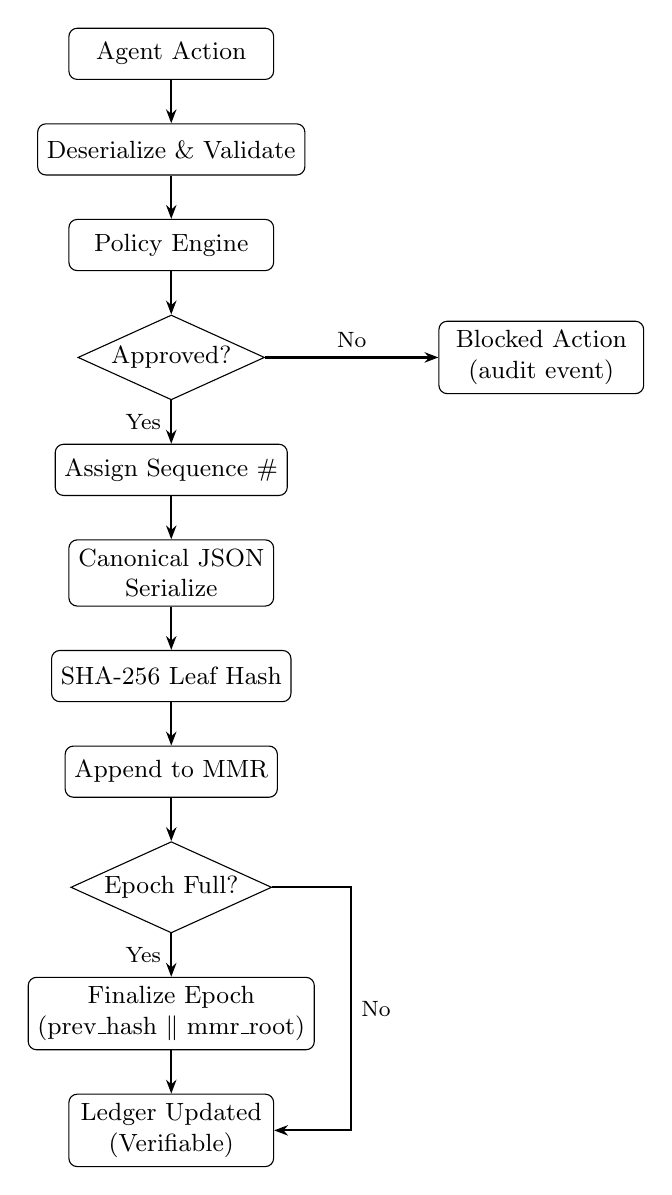
\begin{tikzpicture}[
  node distance=0.55cm and 1.1cm,
  box/.style={rectangle, draw, rounded corners=3pt, minimum width=2.6cm,
              minimum height=0.65cm, font=\small, align=center},
  decision/.style={diamond, draw, aspect=2.2, minimum width=2.2cm,
                   minimum height=0.55cm, font=\small, align=center,
                   inner sep=1pt},
  arr/.style={-{Stealth[length=5pt]}, thick}
]
\node[box] (agent)    {Agent Action};
\node[box, below=of agent]    (deser)   {Deserialize \& Validate};
\node[box, below=of deser]    (policy)  {Policy Engine};
\node[decision, below=of policy] (dec) {Approved?};
\node[box, below=of dec]      (seq)    {Assign Sequence \#};
\node[box, below=of seq]      (canon)  {Canonical JSON\\Serialize};
\node[box, below=of canon]    (hash)   {SHA-256 Leaf Hash};
\node[box, below=of hash]     (mmr)    {Append to MMR};
\node[decision, below=of mmr] (epoch)  {Epoch Full?};
\node[box, below=of epoch]    (fin)    {Finalize Epoch\\(prev\_hash $\|$ mmr\_root)};
\node[box, below=of fin]      (done)   {Ledger Updated\\(Verifiable)};
\node[box, right=2.2cm of dec] (blocked) {Blocked Action\\(audit event)};

\draw[arr] (agent)   -- (deser);
\draw[arr] (deser)   -- (policy);
\draw[arr] (policy)  -- (dec);
\draw[arr] (dec)     -- node[left,font=\footnotesize]{Yes} (seq);
\draw[arr] (dec)     -- node[above,font=\footnotesize]{No} (blocked);
\draw[arr] (seq)     -- (canon);
\draw[arr] (canon)   -- (hash);
\draw[arr] (hash)    -- (mmr);
\draw[arr] (mmr)     -- (epoch);
\draw[arr] (epoch)   -- node[left,font=\footnotesize]{Yes} (fin);
\draw[arr] (fin)     -- (done);
\draw[arr] (epoch.east) -- ++(1.0,0) |- node[right,font=\footnotesize,pos=0.25]{No} (done.east);
\end{tikzpicture}
\caption{LICITRA-MMR two-phase commit pipeline. Phase~1 validates and evaluates
  the proposed action; Phase~2 commits atomically within a single database
  transaction. Epoch finalization chains epoch roots into a hash-linked
  tamper-evident sequence.}
\label{fig:pipeline}
\end{figure}

\subsection{Verification}

An external auditor can verify any historical event independently via three
checks: (1)~\textit{Leaf verification}: recompute the leaf hash and compare to
the stored value; (2)~\textit{Inclusion proof}: verify the MMR proof path
against the epoch root; (3)~\textit{Epoch chain}: recompute each epoch hash from
a trusted anchor and compare to stored values. All three checks require only the
canonical event payload, the epoch's MMR node set, and a single trusted epoch
hash anchor.

%%─────────────────────────────────────────────────────────────────────────────
\section{Implementation}

LICITRA-MMR is implemented in Python~3.11 using FastAPI, SQLAlchemy~2.0, and
PostgreSQL~15. The MMR construction is a custom implementation with no
third-party MMR library dependency; the \texttt{mmr} module implements peak
tracking, node persistence, and inclusion proof generation from first principles.
The implementation is available at
\url{https://github.com/narendrakumarnutalapati/licitra-mmr-core} under MIT
license at tagged release v0.1.0-mvp (commit \texttt{70ec6e4}).

\subsection{Key Design Decisions}

\textbf{MMR recomputed from persisted nodes.} The MMR root is never cached in
application memory. Every MMR operation loads the ordered node list from the
database, ensuring the root always reflects persisted state and any direct
database modification is immediately detectable on the next verification
operation.

\textbf{DEV\_MODE endpoint gating.} Tamper simulation and ledger reset endpoints
return HTTP~403 unless \texttt{DEV\_MODE=true} is explicitly set, with
\texttt{false} as the default. The \texttt{.env} file is excluded from version
control.

\textbf{Atomic transaction boundary.} The commit pipeline uses a single
\texttt{db.commit()} at the pipeline boundary. All intermediate writes use
\texttt{db.flush()} to assign database IDs without committing, ensuring any
failure results in a full rollback with no partial state externally observable.

\textbf{SHA-256 via Python hashlib.} All cryptographic operations use Python's
\texttt{hashlib.sha256}, which wraps OpenSSL. SHA-256 is FIPS~180-4 compliant
and accepted by major compliance frameworks.

\subsection{Test Suite and Evidence Bundles}

The implementation includes 11 passing tests covering: event proposal and
commitment; MMR node persistence and root recomputation; epoch finalization and
hash chaining; T1 payload modification detection; T2 row deletion detection; T3
epoch hash modification detection; T4 cross-epoch chain verification. Five
reproducible evidence scenarios are provided as JSON bundles: S01 (normal
commit), S02 (leaf tamper), S03 (epoch tamper), S04 (row deletion), and S05
(cross-epoch verification).

%%─────────────────────────────────────────────────────────────────────────────
\section{Reproducibility and Artifact}
\label{sec:reproducibility}

\begin{mdframed}[backgroundcolor=gray!7,linewidth=0.6pt,
  innerleftmargin=10pt,innerrightmargin=10pt,
  innertopmargin=8pt,innerbottommargin=8pt]
\noindent
\textbf{Repository:} \url{https://github.com/narendrakumarnutalapati/licitra-mmr-core}\\[2pt]
\textbf{Tagged release:} v0.1.0-mvp \quad|\quad \textbf{Commit hash:} \texttt{70ec6e4}\\
\textbf{Runtime:} Python~3.11, PostgreSQL~15, FastAPI, SQLAlchemy~2.0\\[2pt]
\textbf{Test command:} \texttt{pytest tests/ -v} \quad(11/11 passing at tagged release)\\[2pt]
\textbf{Zenodo code archive:} \url{https://doi.org/10.5281/zenodo.18796529}\\
\textbf{Zenodo paper archive:} \texttt{https://doi.org/10.5281/zenodo.18843032}\\
\textbf{PDF SHA-256:} \texttt{E1A66014E5948712247DD3984CAB0C84C0237BD4D9335E4182AFF01AFD4AC56D}
\end{mdframed}

\medskip
\noindent\textbf{Performance disclaimer.} All performance figures in this report
are analytical estimates derived from SHA-256 microbenchmark component latencies
(Python~3.11 \texttt{hashlib.sha256} via \texttt{timeit}, $\approx$500~ns per
call on Intel x86-64 at 3.2~GHz). They do not include database I/O, network
overhead, connection pool behavior, payload size variance, or cold cache
conditions. No production benchmarking under concurrent workload has yet been
performed. Database I/O dominates the commit path in production; cryptographic
overhead is analytically negligible relative to network and disk latency.
End-to-end profiling under production workloads is an identified future
direction.

%%─────────────────────────────────────────────────────────────────────────────
\section{Comparative Analysis}
\label{sec:comparison}

Table~\ref{tab:comparison} compares LICITRA-MMR against four systems with
related architectural goals, based on publicly documented design properties.

\begin{table}[H]
\centering
\caption{Architectural feature comparison: tamper-evident audit systems for
  agentic AI governance}
\label{tab:comparison}
\begin{tabular}{lcccc}
\toprule
Feature & LICITRA-MMR & immudb & CT Logs & Oktsec \\
\midrule
Data structure           & MMR         & Merkle tree & Merkle tree & Hash chain \\
Inclusion proof          & $O(\log n)$ & $O(\log n)$ & $O(\log n)$ & $O(n)$ \\
Epoch anchoring          & \checkmark  & $\times$    & $\times$    & $\times$ \\
Per-org ledger           & \checkmark  & Partial     & $\times$    & \checkmark \\
Pre-execution gate       & $\times$    & $\times$    & $\times$    & $\times$ \\
Explicit AI audit design & \checkmark  & $\times$    & $\times$    & Partial \\
Canonical JSON spec      & \checkmark  & $\times$    & $\times$    & $\times$ \\
Independent verification & \checkmark  & \checkmark  & \checkmark  & $\times$ \\
License                  & MIT         & Apache-2.0  & N/A         & GPL-3.0 \\
Regulatory alignment    & AI governance/audit & General   & PKI/TLS     & None \\
\bottomrule
\end{tabular}
\end{table}

\textbf{immudb}~\cite{immudb} is a general-purpose tamper-evident database using
a Merkle tree over a linear log, providing inclusion proofs and independent
verification, making it the closest architectural peer. LICITRA-MMR differs from
immudb in three ways material to agentic AI governance: (1)~per-organization
epoch anchoring providing forensic namespace isolation; (2)~a versioned canonical
serialization specification enabling deterministic cross-implementation
verification; and (3)~explicit design alignment with agentic AI governance
requirements, including the two-phase commit pipeline and evidence bundle format.

\textbf{Certificate Transparency logs}~\cite{laurie2013} provide a globally
auditable append-only log for TLS certificates with gossip-based consistency
across independent operators. CT logs address a different problem domain: proving
certificate existence in a publicly auditable multi-operator log. They require
external operators, have no per-organization namespacing, and are not designed
for high-frequency per-organization event streams.

\textbf{Oktsec}~\cite{oktsec} provides agent identity verification and message
integrity using Ed25519 signatures and SHA-256 hash chains. LICITRA-MMR addresses
a complementary layer: epoch-anchored, independently verifiable commitment of
authorized agent decisions, rather than message-level integrity. The primary
structural difference is that a hash chain requires $O(n)$ replay to verify any
historical event, whereas the MMR provides $O(\log n)$ verification of any
single event without full chain replay.

%%─────────────────────────────────────────────────────────────────────────────
\section{Analytical Performance Evaluation}
\label{sec:performance}

\noindent\textit{All figures in this section are analytical estimates. See the
performance disclaimer in Section~\ref{sec:reproducibility}.}

\medskip
All estimates use Python~3.11 \texttt{hashlib.sha256} on an Intel x86-64
processor (3.2~GHz), with SHA-256 latency of approximately 500~ns per call as
measured via \texttt{timeit} microbenchmark. Typical agent event payloads are
assumed to be approximately 200~bytes. Database I/O latency dominates the commit
path; cryptographic overhead is negligible in all scenarios.

\subsection{Inclusion Proof Path Length}

Table~\ref{tab:proof} shows proof path lengths at various epoch sizes. At the
default block size of 1,000, an inclusion proof requires 14 SHA-256 operations
and occupies 462~bytes in binary encoding.

\begin{table}[H]
\centering
\caption{MMR inclusion proof path length by epoch size (confirming $O(\log n)$
  scaling)}
\label{tab:proof}
\begin{tabular}{rrrr}
\toprule
Epoch size & Proof path & MMR nodes & Proof size \\
(events)   & (hashes)   &           & (binary) \\
\midrule
100    &  8 &     197 & 264~B \\
500    & 13 &     994 & 429~B \\
1,000  & 14 &   1,994 & 462~B \\
2,000  & 15 &   3,994 & 495~B \\
10,000 & 17 &  19,995 & 561~B \\
\bottomrule
\end{tabular}
\end{table}

\subsection{Verification Cost at 1 Million Events}

With block size 1,000, one million events produce 1,000 epochs. \textit{Epoch
chain verification} requires 2 SHA-256 operations per epoch (2,000 total),
completing in approximately 1~ms. \textit{Per-event inclusion proof} requires 14
SHA-256 operations and completes in approximately 7~$\mu$s per event.
\textit{Full leaf rehash} of all 1 million events requires approximately
2~seconds at 2~$\mu$s per event. \textit{Sample verification} of 100 randomly
selected events requires approximately 0.9~ms.

\noindent\textit{These figures represent isolated cryptographic computation
time only and do not represent end-to-end system latency. Production latency
will be dominated by database I/O, network round-trips, and connection pool
overhead, none of which are included in these estimates.}

\subsection{Commit Overhead}

The amortized cryptographic overhead per commit is approximately 6 SHA-256
operations ($\approx3~\mu$s). The dominant commit cost is database I/O: three
write operations per commit.

\subsection{Storage at Scale}

At 1 million events with block size 1,000, the estimated storage footprint is
approximately 564~MB: MMR nodes~$\approx$217~MB (1,994,000 node rows), event
rows~$\approx$347~MB (1,000,000 rows at~$\approx$364~bytes each), epoch
rows~$<1$~MB. Storage scales linearly with event count. The MMR node overhead is
approximately $2\times$ the leaf count, consistent with the asymptotic minimum
for append-only binary hash tree constructions.

%%─────────────────────────────────────────────────────────────────────────────
\section{Architectural Non-Goals}
\label{sec:nongoals}

The following properties are explicitly outside the scope of LICITRA-MMR.

\textbf{Not a consensus system.} There is one writer and one ledger per
organization. Consistency is enforced by database transaction semantics, not a
consensus protocol.

\textbf{Not a blockchain.} The epoch chain is structurally similar to a
blockchain header chain but is not a blockchain. There is no proof of work,
proof of stake, token, peer-to-peer network, or distributed ledger.

\textbf{Not Byzantine fault tolerant.} The system assumes the database storage
layer faithfully preserves byte-level fidelity of stored values. It does not
protect against a Byzantine storage layer.

\textbf{Not preventing application-layer falsification.} LICITRA-MMR commits
whatever the application layer submits. Pre-execution authorization integrity is
outside the scope of this system.

\textbf{Not availability-protecting.} Availability is the responsibility of the
deployment infrastructure.

%%─────────────────────────────────────────────────────────────────────────────
\section{Known Limitations}
\label{sec:limitations}

\subsection{Float Normalization Gap}

The canonical JSON specification does not normalize floating-point values. The
integer \texttt{1} and the float \texttt{1.0} produce different byte sequences
and different leaf hashes. For the primary use case of agent decision logging,
this is unlikely to cause verification failures in practice, provided callers
ensure consistent numeric types. Full float normalization per RFC~8785~\S3.2.2
is an identified future extension for CANONICAL\_JSON\_SPEC~v1.1.

\subsection{Unsigned Epoch Roots}

The current implementation computes epoch hashes but does not sign them with a
private key. An attacker who controls both the database and the application
server can in principle reconstruct a consistent but false history. Ed25519 epoch
signing is an identified future extension. The epoch record schema reserves a
\texttt{signature} field for this purpose.

\subsection{Single-Operator Trust Model}

LICITRA-MMR is designed for single-operator deployments. Multi-party
witnessing---where multiple independent operators each hold a copy of the current
epoch hash---is an identified future architectural direction, analogous to the
gossip protocol in Certificate Transparency~\cite{laurie2013}.

\subsection{Pre-Execution Integrity}

LICITRA-MMR records what was committed. It does not guarantee that what was
committed accurately reflects what the agent was authorized to do. Pre-execution
authorization integrity is outside the scope of this system.

\subsection{Production Profiling}

All performance figures in this report are analytical estimates. End-to-end
profiling under production workloads---including p50/p95 latency distributions,
cold versus warm cache conditions, and database I/O breakdown---is an identified
future direction.

%%─────────────────────────────────────────────────────────────────────────────
\section{Related Work}

\textbf{Merkle Mountain Ranges.} MMRs were introduced by Peter
Todd~\cite{todd2013} and have been adopted in blockchain systems including Grin
and Beam. The formal optimality of the MMR for append-only accumulators was
established by Bonneau et al.~\cite{bonneau2025}. To the author's knowledge,
prior literature has not explicitly applied MMR structures to per-organization
agentic AI audit logs.

\textbf{Certificate Transparency.} Laurie et al.~\cite{laurie2013} introduced CT
logs for publicly auditing TLS certificate issuance. LICITRA-MMR shares the
append-only authenticated structure but differs in trust model, scope, and
operational requirements.

\textbf{immudb.} Codenotary's immudb~\cite{immudb} provides a tamper-evident
database using a Merkle tree over an append-only log. It is the closest
architectural peer; distinctions are described in Section~\ref{sec:comparison}.

\textbf{Oktsec.} The Oktsec framework~\cite{oktsec} provides agent identity
verification and message integrity. LICITRA-MMR addresses a complementary layer
at the authorization record and audit level.

\textbf{NIST AI Risk Management Framework.} The NIST AI RMF~\cite{nistai}
provides governance guidance including auditability requirements. LICITRA-MMR
provides a technical implementation component consistent with that guidance.

%%─────────────────────────────────────────────────────────────────────────────
\section{Conclusion}

This report has documented LICITRA-MMR, an open-source cryptographic ledger
primitive for agentic AI runtime accountability. The system combines a Merkle
Mountain Range with per-organization epoch anchoring, a versioned canonical JSON
specification, and an atomic two-phase commit pipeline to provide forensic
integrity guarantees that mutable logging infrastructure does not offer.

The three core contributions---the canonical specification, the MMR-based
epoch-anchored ledger, and the atomic commit pipeline---address the gap between
what emerging AI regulation implies (post-incident reconstructability with
sufficient integrity for audit) and what most production agentic AI stacks
currently provide (operator-controlled mutable logs).

\subsection{Deployment Considerations}

Organizations deploying LICITRA-MMR should consider:
(1)~\textit{Epoch hash anchoring}---store at least one epoch hash off-site via a
notarization service, timestamping service, or publication to a public ledger,
to prevent an operator from reconstructing a consistent false history;
(2)~\textit{Key management preparation}---establish KMS or HSM infrastructure in
advance of implementing Ed25519 epoch signing;
(3)~\textit{Backup and retention}---the MMR node table grows at approximately
$2\times$ the event count;
(4)~\textit{Regulatory export}---use the JSON evidence bundle format from the
\texttt{licitra-mmr-evidence} repository for regulatory submissions.

\bigskip
\noindent\textbf{Reproducibility.} All code, test suites, and evidence bundles
are available at
\url{https://github.com/narendrakumarnutalapati/licitra-mmr-core}. The tagged
release v0.1.0-mvp (commit \texttt{70ec6e4}) and all evidence bundles are
permanently archived at \url{https://doi.org/10.5281/zenodo.18796529} (code
repository). This report is archived at \texttt{https://doi.org/10.5281/zenodo.18843032}.

%%─────────────────────────────────────────────────────────────────────────────
\section*{Suggested Citation}

\begin{quote}
\small
Nutalapati, N.K. (2026). \emph{LICITRA-MMR: A Merkle Mountain Range Ledger Primitive for
Cryptographic Runtime Accountability in Agentic AI Systems}. LICITRA Technical Report Series,
Report No.\ LICITRA-TR-2026-01, Version~0.2.
Zenodo. \url{https://doi.org/10.5281/zenodo.18843032}
\end{quote}

BibTeX:
\begin{verbatim}
@techreport{licitrammr2026,
  author      = {Nutalapati, Narendra Kumar},
  title       = {{LICITRA-MMR}: A Merkle Mountain Range
                 Ledger Primitive for Cryptographic
                 Runtime Accountability in Agentic
                 {AI} Systems},
  number      = {LICITRA-TR-2026-01},
  version     = {0.2},
  year        = {2026},
  month       = mar,
  doi         = {10.5281/zenodo.18843032},
  url         = {https://doi.org/10.5281/zenodo.
                 18843032},
  institution = {LICITRA Technical Report Series},
}
\end{verbatim}

%%─────────────────────────────────────────────────────────────────────────────
\section*{Version History}

\begin{tabular}{@{}llp{8cm}@{}}
\toprule
\textbf{Version} & \textbf{Date} & \textbf{Summary} \\
\midrule
0.1 & February 2026 & Initial MVP: MMR implementation, 11/11 tests,
evidence bundles S01--S05, Zenodo code archive. \\
0.2 & March 2026 & Formalized threat model, security property statements,
explicit scope limitations, analytical performance section with disclaimer.
Restructured as LICITRA-TR-2026-01 under the LICITRA Technical Report Series.
Updated artifact metadata, suggested citation with BibTeX, and license split
(MIT code, CC~BY~4.0 report). Added cross-reference to companion report
LICITRA-TR-2026-02 (LICITRA-SENTRY). \\
\bottomrule
\end{tabular}

\medskip
\noindent\textit{Note on versioning convention.} The version number of this
technical report (v0.2) tracks documentation maturity independently of the
software release number. Version~0.1 refers to the software implementation
artifact, released as tagged release \texttt{v0.1.0-mvp} in February~2026 and
permanently archived at
\url{https://doi.org/10.5281/zenodo.18796529}. This report (v0.2) documents,
formalizes, and analyzes that implementation. The two artifacts---software
and technical report---are archived separately on Zenodo under the LICITRA
Technical Report Series.

%%─────────────────────────────────────────────────────────────────────────────
\bibliographystyle{plain}
\begin{thebibliography}{9}

\bibitem{todd2013}
P.~Todd.
\newblock Merkle Mountain Ranges.
\newblock OpenTimestamps, 2013.
\newblock \url{https://github.com/opentimestamps/opentimestamps-server/blob/master/doc/merkle-mountain-range.md}

\bibitem{laurie2013}
B.~Laurie, A.~Langley, and E.~Kasper.
\newblock Certificate Transparency.
\newblock RFC~6962, Internet Engineering Task Force, 2013.
\newblock \url{https://www.rfc-editor.org/rfc/rfc6962}

\bibitem{bonneau2025}
J.~Bonneau, J.~Chen, M.~Christ, and I.~Karantaidou.
\newblock Merkle Mountain Ranges are Optimal: On Witness Update Frequency for
  Cryptographic Accumulators.
\newblock In \textit{Advances in Cryptology -- CRYPTO~2025}, LNCS vol.~16001,
  Springer, 2025.
\newblock \url{https://eprint.iacr.org/2025/234}

\bibitem{immudb}
Codenotary.
\newblock immudb: Immutable Database.
\newblock \url{https://immudb.io}

\bibitem{oktsec}
Oktsec.
\newblock Agent Security Framework (v0.1).
\newblock \url{https://github.com/oktsec/oktsec}
\newblock Accessed: February 2026.

\bibitem{nistai}
National Institute of Standards and Technology.
\newblock Artificial Intelligence Risk Management Framework (AI~RMF~1.0).
\newblock \url{https://doi.org/10.6028/NIST.AI.100-1}, 2023.

\bibitem{euaiact}
European Parliament.
\newblock Regulation (EU) 2024/1689 on Artificial Intelligence (EU AI Act).
\newblock Official Journal of the European Union, 2024.

\bibitem{coloradoai}
Colorado General Assembly.
\newblock SB~24-205: Colorado Artificial Intelligence Act.
\newblock Effective June~30, 2026.
\newblock \url{https://leg.colorado.gov/bills/sb24-205}

\bibitem{licitrasentry}
N.~K.~Nutalapati.
\newblock LICITRA-SENTRY: Deterministic Inter-Agent Authorization Control Plane
  with Cryptographic Audit Integrity.
\newblock LICITRA Technical Report Series, Report No.\ LICITRA-TR-2026-02,
  Version~0.1, Zenodo, March 2026.
\newblock DOI: \url{https://doi.org/10.5281/zenodo.18843784}.
\newblock Code archive: \url{https://doi.org/10.5281/zenodo.18843592}.

\end{thebibliography}

\end{document}
